\section{Algoritmo}

Utilizzando le tecniche descritte nella sezione precedente è stato ideato l'algoritmo descritto in [1].

L'algoritmo può essere suddiviso in 4 parti fondamentali:
\begin{enumerate}
\item Creazione dei filtri di Gabor
\item Estrazione di features
\item Creazione di un modello a mistura di gaussiane
\item Calcolo dei \emph{tensori di fisher}
\item Classificazione
\end{enumerate}

Inizialmente viene creato il set di filtri di Gabor, impostando 4 diverse orientazioni e 3 diverse scale. Si ottengono così 12 filtri distinti che verranno utilizzati nella fase di estrazione delle \emph{features}.

\subsection{Estrazione delle \emph{features}}

In questa fase ciascuna scansione viene elaborata al fine di estrarre delle \emph{features}. 

Inizialmente, data un immagine viene calcolata la sua maschera, ovvero un'immagine binaria che evidenzia i pixels di \emph{foreground}. In questo modo il calcolo delle \emph{features} verrà effettuato solamente sui pixels rilevanti dell'immagine, escludendo lo sfondo. La maschera viene calcolata mediante un'operazione di sogliatura tramite il metodo di Otsu.

L'immagine viene scansionata a blocchi quadrati di dimensione 80 pixels, sovrapposti con un passo di 20 pixels.

\begin{figure}[H]
\captionsetup[subfigure]{labelformat=empty}
\begin{subfigure}{.5\textwidth}
\centering
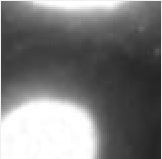
\includegraphics[height=1.6cm]{images/block.png}
\caption{Blocco}
\end{subfigure}%
\begin{subfigure}{.5\textwidth}
\centering
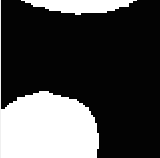
\includegraphics[height=1.8cm]{images/mask.png}
\caption{Maschera}
\end{subfigure}%
\caption{Esempio di blocco e maschera di elaborazione}
\end{figure}

A questo punto, considerando solo i pixel del blocco filtrati dalla maschera, per ciascun pixel viene estratto un vettore di 15 osservazioni così composto:

$$F_{x,y} = [I(x, y), x, y, |G_{0,0}(x, y)|, \ldots, |G_{0, v}(x, y)|, |G_{1, 0}(x, y)|, \ldots, |G_{u, v}(x, y)|]$$

dove 
\begin{itemize}
\item $I(x, y)$ è il livello di grigio del pixel alla posizione $(x, y)$.
\item $x, y$ solo rispettivamente l'ascissa e l'ordinata del pixel considerato.
\item $u$ è il numero delle scale del filtro di Gabor (in questo caso 3).
\item $v$ è il numero delle orientazioni del filtro di Gabor (in questo caso 4).
\end{itemize}

A questo punto a ciascun pixel del blocco è associato un vettore di 15 osservazioni, dunque la matrice delle \emph{features} avrà dimensione $15\; X\; n^2$, con $n$ dimensione del blocco (in questo caso 80).
Si procede dunque con il calcolo del \emph{descrittore di covarianza} del blocco, ottenendo una matrice $C$ di dimensione $15 \; X \; 15$.

Gli elementi della diagonale di questa matrice rappresentano le varianze di ciascuna osservazione e gli elementi extra diagonali rappresentano le correlazioni. 

In ultima istanza viene effettuato il \emph{mapping} sullo spazio tangente per ricondurci alla geometria Riemanniana.

\begin{figure}[H] 
  \centering
    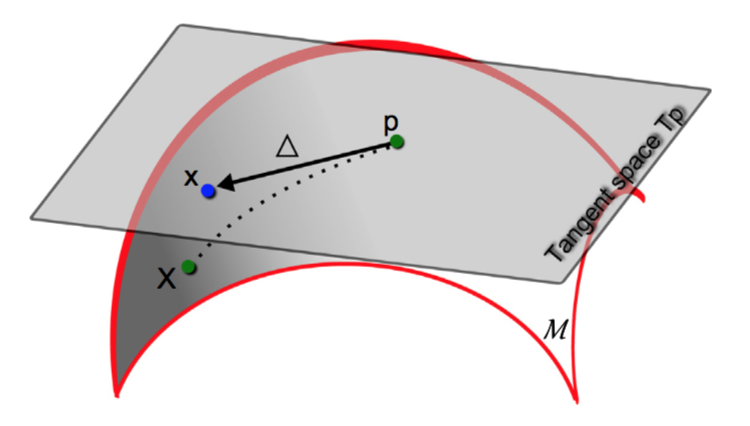
\includegraphics[width=0.5\textwidth]{images/tangent_space.png}
    \caption{{\textit{Illustrazione dello spazio tangente $T_P$ al punto $P$ sulla varietà Riemanniana $\mathcal{M}$}}}
\end{figure}

Il vettore tangente $\Delta$ può essere ottenuto mediante mappa logaritmica, $\Delta = \log(C)$.

\subsection{Creazione di un modello a mistura di gaussiane}

